\chapter{Conceptual Design}
Ein erstes Design für die Benutzeroberfläche wurde mit dem Mockup Tool \textit{Balsamiq} entwickelt. Hierbei ging es primär darum Unstimmigkeiten und grobe Fehleinschätzungen auszumerzen, um anschließend einen funktionalen Prototypen entwickeln zu können. Mehr oder weniger parallel wurden auch schon Mock-Ups mit Hilfe von HTML erzeugt, welche den Vorteil hatten, später weiter genutzt werden zu können, da für die Umsetzung der App hauptsächlich HTML5 und JavaScript zum Einsatz kam.

Auf den folgenden Bildern sind die \textit{Balsamiq} Mock-Ups und die ggf. verschiedenen Versionen der App Umsetzung bzw. der HTML Mock-Ups zu sehen:

\subsubsection*{Mockups}
\begin{figure}[ht]
\centering
\begin{minipage}[b]{.5\textwidth}
  \centering
  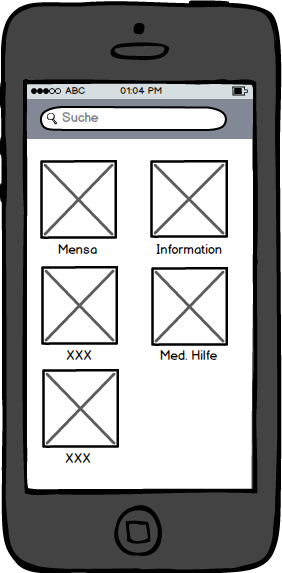
\includegraphics[width=.8\linewidth]{img/menu-mockup.png}
  \label{img:menu-mockup}
  \captionof{figure}{Menü Mockup}
\end{minipage}%
\begin{minipage}[b]{.5\textwidth}
  \centering
  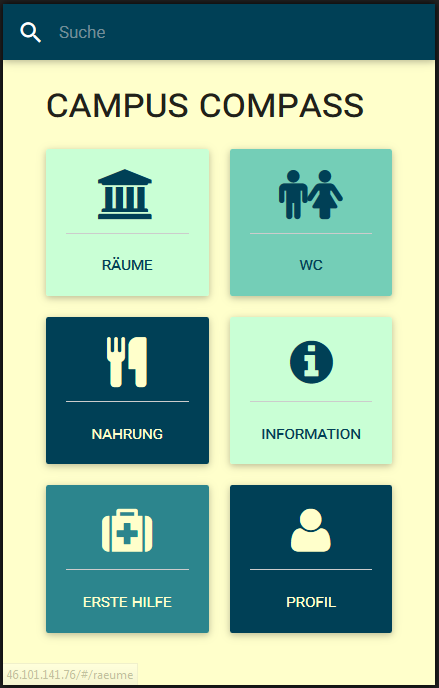
\includegraphics[width=.8\linewidth]{img/menu.png}
  \label{img:menu-first-draft}
  \captionof{figure}{Erster Entwurf Menü}
\end{minipage}
\end{figure}

\begin{figure}[ht]
\centering
\begin{minipage}[b]{.5\textwidth}
  \centering
  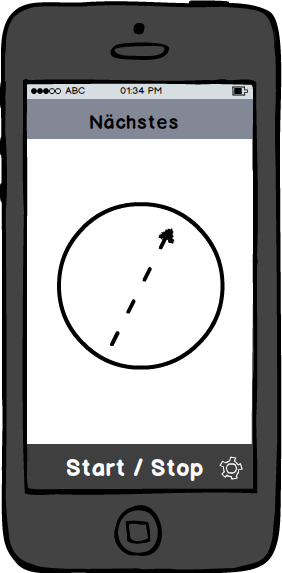
\includegraphics[width=.8\linewidth]{img/navigation-mockup.png}
  \label{img:navigation-mockup}
  \captionof{figure}{\gls{navigation} Mockup}
\end{minipage}%
\begin{minipage}[b]{.5\textwidth}
  \centering
  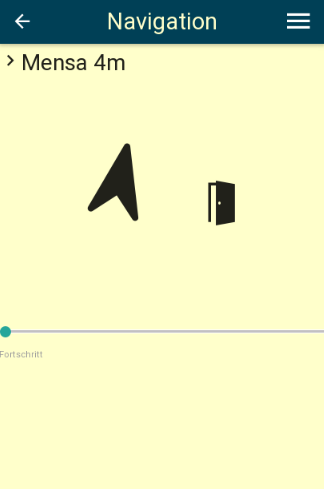
\includegraphics[width=.8\linewidth]{img/navigation.png}
  \label{img:navigation-first-draft}
  \captionof{figure}{Erster Entwurf \gls{navigation}}
\end{minipage}
\begin{minipage}[b]{.5\textwidth}
  \centering
  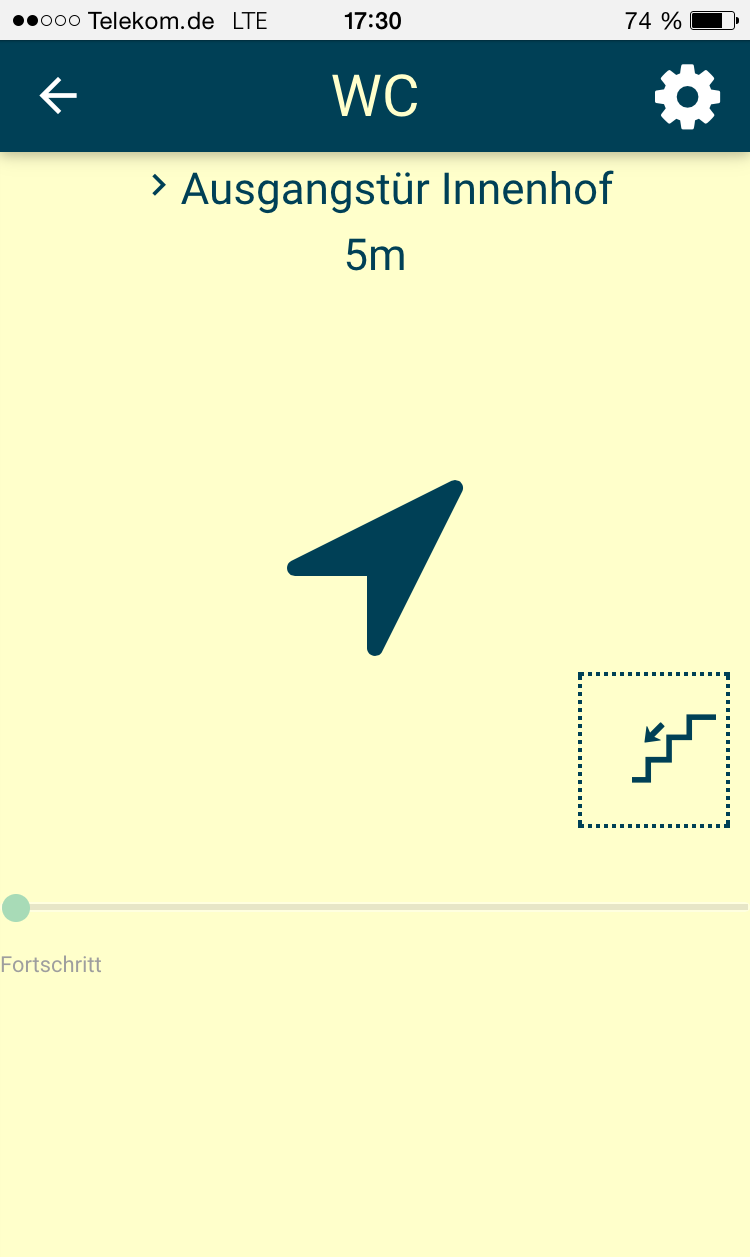
\includegraphics[width=.8\linewidth]{img/navigation2.png}
  \label{img:navigation-second-draft}
  \captionof{figure}{Aktuelle Ansicht \gls{navigation}}
\end{minipage}
\end{figure}

\begin{figure}[ht]
\centering
\begin{minipage}[b]{.5\textwidth}
  \centering
  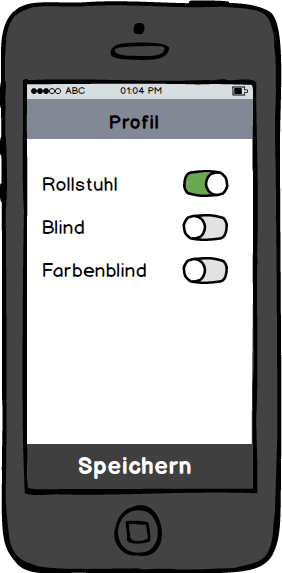
\includegraphics[width=.8\linewidth]{img/profil-mockup.png}
  \label{img:profil-mockup}
  \captionof{figure}{Profil Mockup}
\end{minipage}%
\begin{minipage}[b]{.5\textwidth}
  \centering
  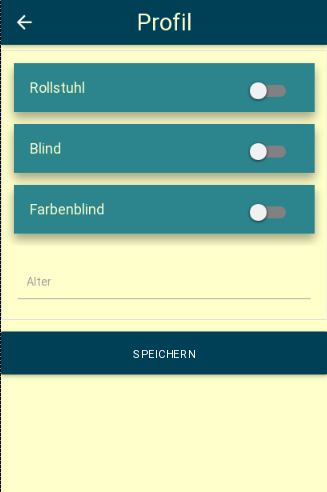
\includegraphics[width=.8\linewidth]{img/profil.png}
  \label{img:profil-first-draft}
  \captionof{figure}{Erster Entwurf Profil}
\end{minipage}
\end{figure}

\begin{figure}[ht]
\centering
\begin{minipage}[b]{.5\textwidth}
  \centering
  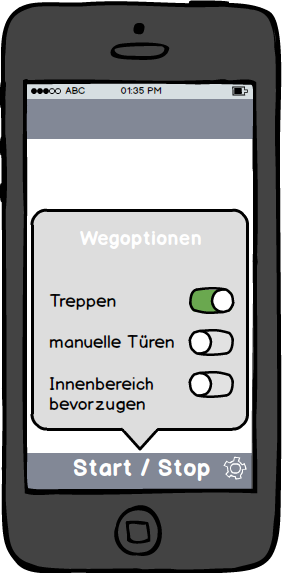
\includegraphics[width=.8\linewidth]{img/wegoptionen-mockup.png}
  \label{img:wegoptionen-mockup}
  \captionof{figure}{\gls{weg}optionen Mockup}
\end{minipage}%
\begin{minipage}[b]{.5\textwidth}
  \centering
  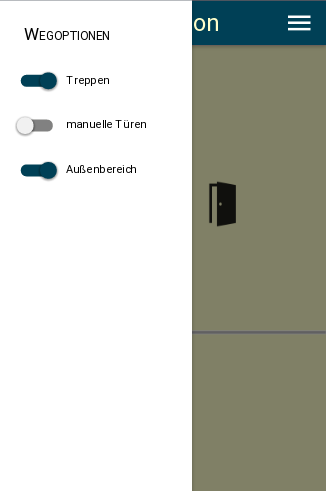
\includegraphics[width=.8\linewidth]{img/wegoptionen.png}
  \label{img:wegoptionen-first-draft}
  \captionof{figure}{Erster Entwurf \gls{weg}optionen}
\end{minipage}
\end{figure}